\chapter{基础知识}
\label{ch2}
在本章节中我们将介绍本文研究所需要的一些基本知识,有助于更好的理解之后章节的内容。

\section{神经网络}
\subsection{基本结构}
深度学习模型通常采用神经网络的形式。已经为不同的应用提出了各种神经网络架构,例如多层感知器、卷积神经网络和循环神经网络。神经网络\upcite{ref34}最初的设计灵感来源于人脑的结构。我们知道,人类的大脑是处理信息的主要部分,也是人中枢神经系统中的重要部分。人脑中含有大量的神经元,它们像网状物一样复杂的相互连接。当人脑接收到外部环境或者感觉器官传入的刺激(兴奋),它随着神经元一层一层的将刺激(兴奋)传导到神经中枢(大脑或脊髓),神经中枢根据接收到的信号,作出不同的判断,最后传递到输出神经。
不同的信号,大脑都可以进行学习和分辨,而这一通用的模型,就是神经网络。

神经网络的基本组成单元是神经元,一个神经网络可能包含数百亿个简单的神经元,它们按层排列,密集而复杂的相互连接着。神经网络中每一层有多个神经元,层与层之间是“前馈传播”的,也就是说,网络中的数据只在一个方向上移动。一个单独的神经元可能与它前面一层的几个神经元相连,它从这些神经元接收数据;与它后面一层的几个神经元相连,它向这些神经元发送数据。每一层的神经元只有可能与其前一层和后一层的神经元相连接,不存在跨层连接。

\begin{figure}[!hbt]
\centering
	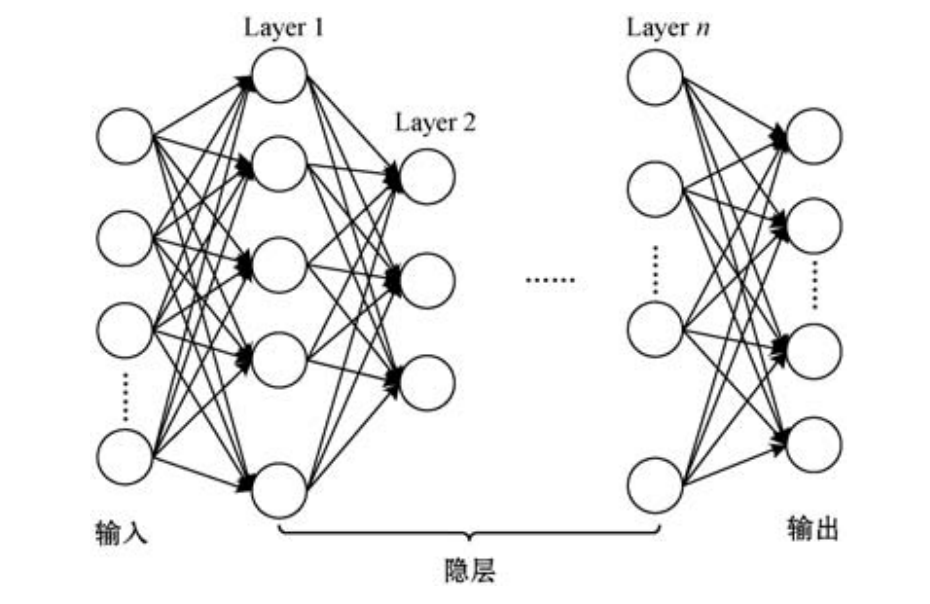
\includegraphics[scale=0.5]{fig2/C2/深度神经网络结构图}%联邦学习的系统架构
	\caption{神经网络结构图}
	\label{fig:神经网络结构图}	
\end{figure}

如图\ref{fig:神经网络结构图}所示,一个神经网络由一个输入层、一个输出层以及输入和输出之间的一系列隐藏层组成。每一层都是一组称为神经元的单元,它们连接到上一层和下一层的其他神经元。输入层用于接收信息,当一个神经网络被训练时,其所有的权重和阈值最初都被设置为随机值,然后训练数据被送入输入层;之后传入隐藏层进行特征的提取、网络权重的调整使得隐藏层的神经单元对某种模式形成反应;最后传导到输出层,输出模型判断的结果。神经元之间的每个连接都可以通过应用线性函数和元素级非线性激活函数(例如 sigmoid 或 ReLU)将信号传输到下一层的另一个神经元。通过这种方式,神经网络通过隐藏层转换输入,然后转换输出。

反向传播和随机梯度下降是训练深度学习模型和寻找最佳参数的常用方法。在深度神经网络中,对每个训练样本,通过前向传播算法从输入层、隐藏层到输出层依次训练,在输出层得到预测的结果,然后根据损失函数计算预测值与真实值之间的差异程度,之后根据反向传播算法调整权重系数,更新网络参数,使得损失函数的值最小,模型达到全局最优。

\subsection{随机梯度下降算法}
随机梯度下降算法(Stochastic Gradient Descent,SGD)是一种主流的用于机器学习和深度学习模型优化的迭代方法,从随机的权重系数开始,迭代运行梯度下降算法,使损失函数收敛到局部最小值,以找到使模型达到全局最优的权重系数,具体的算法如所示。

\begin{algorithm}[!htb]
	\caption{随机梯度下降算法}
	\label{随机梯度下降算法}
	\begin{algorithmic}[1]
		\footnotesize
		\STATE \textbf{输入:} 学习率$\alpha$
		\STATE \textbf{输出:} 初始参数$\theta$
		\STATE 初始化模型权重$\theta$,作为梯度下降的起始点
		\WHILE{模型未达到全局最优点}
		\STATE 从训练集中均匀抽出一小批量(minibatch)样本:$\mathbb{B}=\left\{x^{(1)}, \ldots, x^{\left(m^{\prime}\right)}\right\}$
		\STATE 计算梯度估计:$$
g=\frac{1}{m^{\prime}} \nabla_{\theta} \sum_{i=1}^{m^{\prime}} L\left(x^{(i)}, y^{(i)}, \theta\right)
$$
		\STATE 梯度下降:$$
\theta=\theta-\epsilon g
$$
		\ENDWHILE
	\end{algorithmic}
\end{algorithm}

\subsection{经验风险最小化}
在神经网络中,模型通过不断的学习数据集中的特征得到预测值,通过损失函数计算预测值与真实值之间的误差,之后再采用反向传播算法调整权重系数使得最终的损失函数的值最小。整个模型训练的过程可以理解为经验风险最小化(Empirical risk minimization,ERM)问题:
\begin{equation}\label{eq:ERM}
F(\boldsymbol{\theta}):=\frac{1}{n} \sum_{i=1}^{n} f_{i}(\boldsymbol{\theta})
\end{equation}

模型在训练集$S=$ $\left\{\left(\mathbf{x}_{1}, y_{1}\right), \ldots,\left(\mathbf{x}_{n}, y_{n}\right)\right\}$上进行训练,其中,$F(\boldsymbol{\theta})$表示经验损失函数;$f_{i}(\boldsymbol{\theta})=\ell\left(\boldsymbol{\theta} ; \mathbf{x}_{i}, y_{i}\right)$表示在第$i$个训练样本$\left(\mathbf{x}_{i}, y_{i}\right)$上定义的损失函数;$\boldsymbol{\theta} \in \mathbb{R}^{d}$表示模型最终训练得到的权重参数。模型的训练目标是找到最终的权重参数$\widehat{\boldsymbol{\theta}} \in \mathbb{R}^{d}$ ,使得公式\ref{eq:ERM}所计算得到的经验风险值最小。

\begin{define}\label{全局最优点}
当$\|\nabla f(\boldsymbol{\theta})\|_{2} \leq \zeta$时,$\boldsymbol{\theta} \in \mathbb{R}^{d}$是使得ERM函数达到全局最优解的参数
\end{define}

\begin{define}\label{G-Lipschitz}
对于函数$f$:$\mathbb{R}^{d} \rightarrow \mathbb{R}$,如果对于任意的$\boldsymbol{\theta}_{1}, \boldsymbol{\theta}_{2} \in \mathbb{R}^{d}$,都有$\left|f\left(\boldsymbol{\theta}_{1}\right)-f\left(\boldsymbol{\theta}_{2}\right)\right| \leq G\left\|\boldsymbol{\theta}_{1}-\boldsymbol{\theta}_{2}\right\|_{2}$
,则称函数$f$满足G-Lipschitz(G-利普希茨连续条件)。
\end{define}

\begin{define}\label{L-Lipschitz}
对于函数$f$:$\mathbb{R}^{d} \rightarrow \mathbb{R}$,如果对于任意的$\boldsymbol{\theta}_{1}, \boldsymbol{\theta}_{2} \in \mathbb{R}^{d}$,都有\\$\left\|\nabla f\left(\boldsymbol{\theta}_{1}\right)-\nabla f\left(\boldsymbol{\theta}_{2}\right)\right\|_{2} \leq L\left\|\boldsymbol{\theta}_{1}-\boldsymbol{\theta}_{2}\right\|_{2}$,则称函数$f$满足L-Lipschitz(L-利普希茨连续条件)。
\end{define}

\section{联邦学习}
传统的集中式深度学习需要将训练数据放在一起到数据中心。该模型以集中方式进行训练。而联邦学习允许数据所有者拥有一个私人学习网络,该网络使用本地数据集进行训练。之后,每个参与者将本地模型的梯度上传到云服务器。通过使用云服务器收集的全局梯度进行更新,可以避免局部模型过度拟合。此外,它还保护本地数据不被其他参与者或云服务器直接知道。联邦学习的基本工作流程如下:
\begin{itemize}
\item \textbf{初始化:}
所有用户在个字的设备上都有一个预先分配的神经网络模型,并且可以自愿加入联邦学习协议,指定相同的深度学习和模型训练目标。
\item  \textbf{本地训练:}在一个给定的通信回合中,联邦学习参与者首先从中央服务器下载全局模型参数,然后在各自的本地数据集$D_{i}$上进行模型训练,更新模型参数:$\omega_{i}^{r+1} \leftarrow \omega_{i}^{r}-\eta_{i} \nabla g\left(D_{i}^{t}, \omega_{i}^{r}\right)$
\item \textbf{中央参数聚合:}中央服务器等待所有本地客户端将更新后的模型参数$M1,M2....M_{n}$上传,聚合得到全局模型的参数,之后更新全局模型:$\omega^{r+1} \leftarrow \omega^{r}-\eta \frac{\sum_{U_{i} \in U^{t}} \varsigma U_{i}}{\sum_{U_{i} \in U^{t}}\left|D_{i}^{t}\right|}$
\item \textbf{迭代更新:}迭代地执行上述步骤直至全局模型参数满足收敛条件,最终得到最优的全局模型。
\end{itemize}

\begin{figure}[!hbt]
\centering
	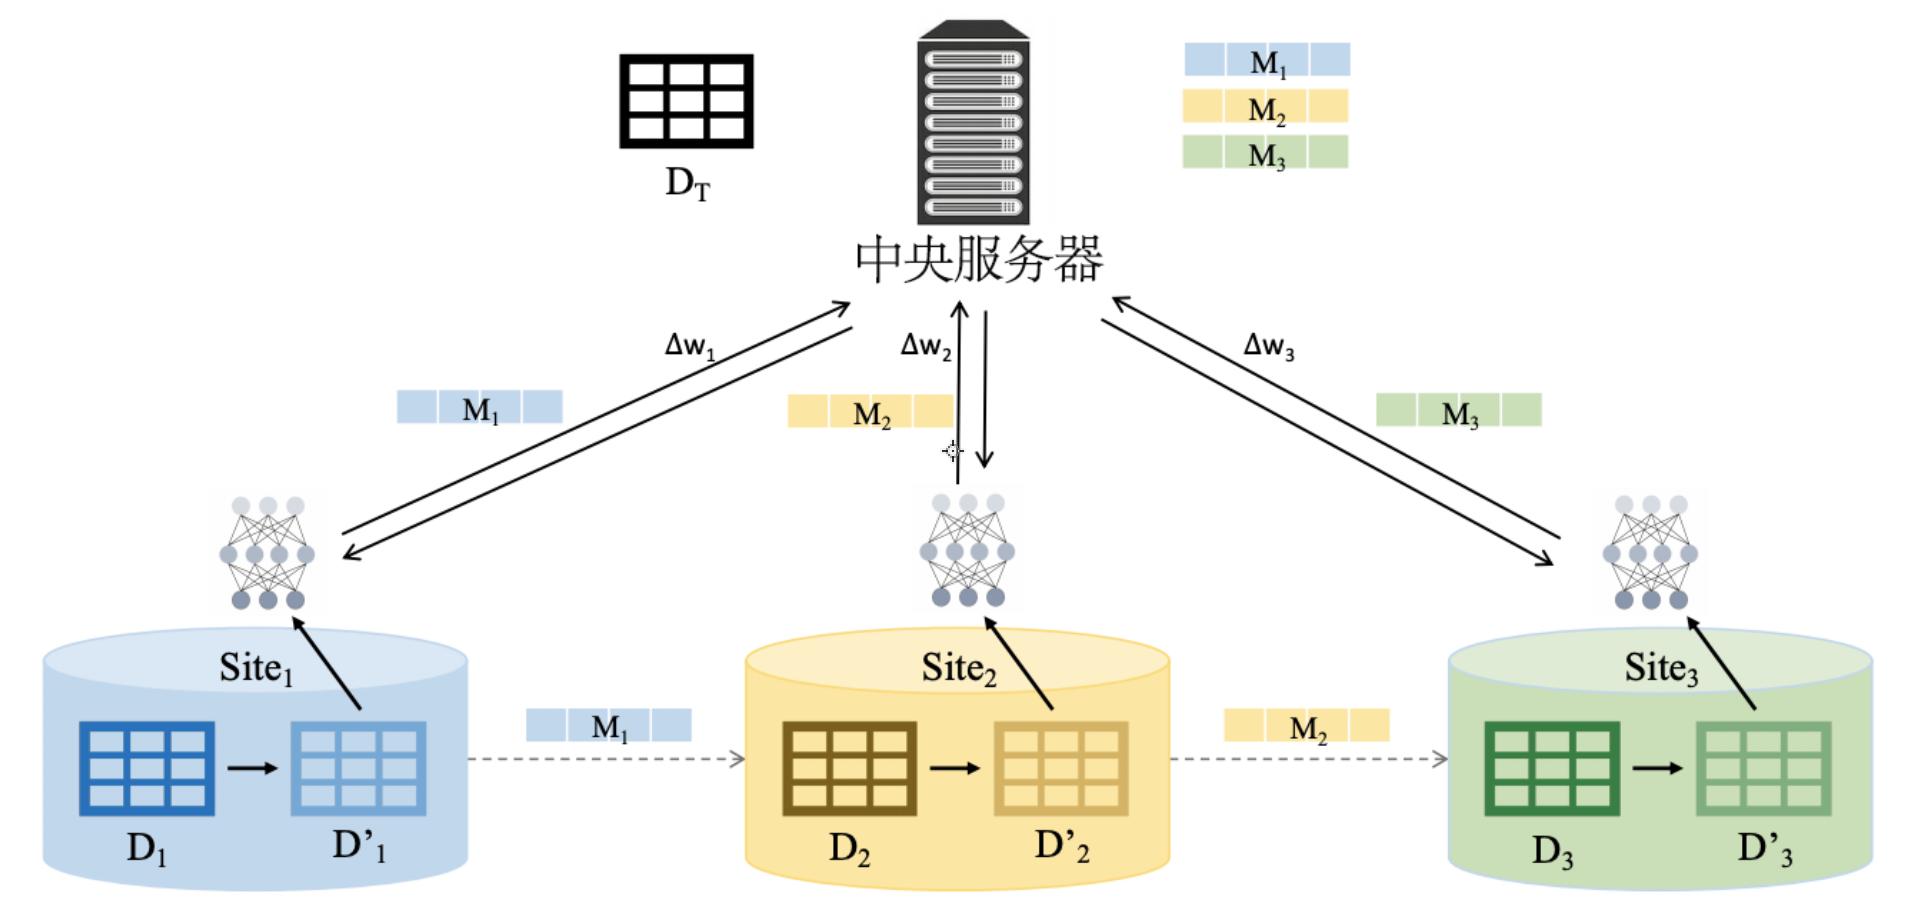
\includegraphics[scale=0.45]{fig2/C2/联邦学习模型流程}%联邦学习的系统架构
	\caption{联邦学习模型工作流程}
	\label{fig:联邦学习模型工作流程}	
\end{figure}

\section{差分隐私}
\subsection{基本定义}
\begin{define}[邻近数据集]\label{邻近数据集}
现有两个属性相近的数据集$D$和$D^{\prime}$,他们的数据记录差为$D \Delta D^{\prime}$,如果$\left|D \Delta D^{\prime}\right|=1$,则称数据集$D$和$D^{\prime}$为邻近数据集(Adjacent Dataset)。
\end{define}

\begin{figure}[!hbt]
\centering
	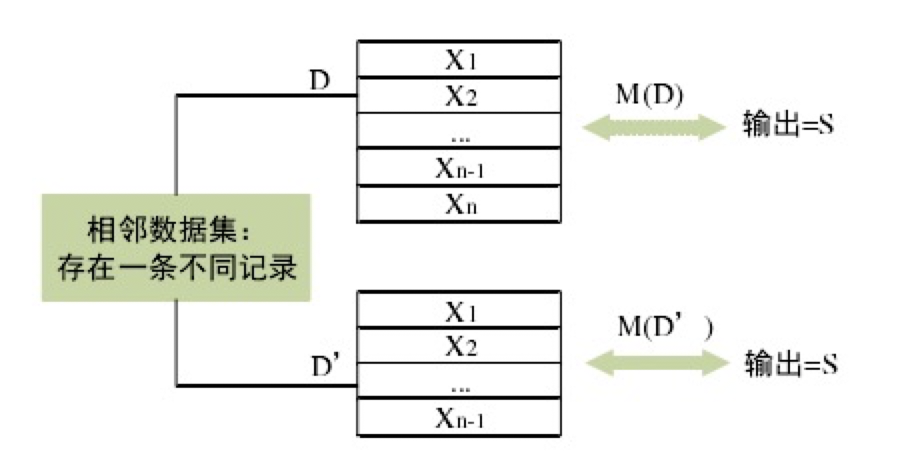
\includegraphics[scale=0.6]{fig2/C2/相邻数据集示意图}%联邦学习的系统架构
	\caption{差分隐私的相邻数据集示意图}
	\label{fig:相邻数据集示意图}	
\end{figure}

2016年,Dwork\upcite{ref14}等人首次提出了差分隐私的概念,它在针对数据隐私泄漏的新型隐私定义,目的是使数据库的查询函数对数据集中单条记录的变化不敏感。其思想是添加一定量的噪音来随机化给定算法的输出,从而使攻击者无法区分任何两个相邻的输入数据集的输出。具体的定义如下:
\begin{define}[(ε,δ)-差分隐私]\label{(ε,δ)-差分隐私}
$\mathcal{D}$表示数据集合,$D$和$D^{\prime}$ 为邻近数据集。现有随机算法$M: D \rightarrow R$,D表示定义域,R表示值域。如果对于任意两个邻近数据集$S, S^{\prime} \in \mathcal{S}^{n}$和输出子集$O \subseteq \mathcal{R}$时,总有$$
\operatorname{Pr}[\mathcal{M}(D) \in S] \leq e^{\epsilon} \operatorname{Pr}\left[\mathcal{M}\left(D^{\prime}\right) \in S\right]+\delta
$$,则称该随机算法满足 $(\varepsilon, \delta)$-差分隐私。
\end{define}
添加项$\delta \in[0,1]$表示以某种概率打破$(\epsilon, 0)$-差分隐私。当$\delta=0$时,则将$M$称为$\epsilon$-差分隐私。$\epsilon$和$\delta$表示隐私预算参数,$\epsilon$和$\delta$越小,算法能提供的隐私保证程度越强。

差分隐私保护的实现是在查询函数的返回值中注入一定量的干扰噪声,但是注入的噪声量太大会影响最终结果的准确性,太少则无法保障数据的隐私性。那么如何衡量添加的噪声量,既能保障数据的安全,又能维持数据的可用性呢?这里针对数据集提出敏感度的概念,加入的噪声量大小与数据集的敏感度息息相关。对于相邻数据集$D$和$D^{\prime}$,他们的敏感度代表某一个查询函数在这两个相邻数据集上输出的最大不同。查询函数的类型决定了敏感度,也为噪声的添加提供了依据。

\begin{define}[全局敏感度]\label{全局敏感度}
假设存在函数 $f: D \rightarrow R^{d}$, 输入为一数据集,输出为$d$维的实数向量。 对于任意的邻近数据集 $D$ 和 $D^{\prime}$,
$$
G S_{f}=\max _{D, D^{\prime}}\left\|f(D)-f\left(D^{\prime}\right)\right\|_{1}
$$
称为函数 $f$ 的全局敏感度。
\end{define}

\subsection{实现机制}
在差分隐私的实际应用中,如何针对不同的场景和问题设计添加噪声的机制使算法能满足差分隐私保护的要求呢?差分隐私的实现机制主要分为拉普拉斯机制(Lapalace Mechanism)\upcite{ref9}、指数机制(Exponential Mechanism)\upcite{ref32}与高斯机制(Gaussian Mechanism)\upcite{ref33}。其中,指数机制适用于非数值型结果的隐私保护,拉普拉斯机制和高斯机制适用于对数值型结果的隐私保护\upcite{ref35}。

\begin{theorem}[拉普拉斯机制]\label{拉普拉斯机制}
给定一个基于数据集$D$的查询函数$f(D)$,算法$\ddot{f}(D)$满足 $\varepsilon$-差分隐私, 当:
$$
\ddot{f}(D)=f(D)+\operatorname{Lap}\left(\frac{G S}{\epsilon}\right)
$$
\end{theorem}
其中,噪声参数满足$\operatorname{Lap}\left(\frac{G S}{\epsilon}\right)$的 Laplace 分布,$GS$表示数据集的敏感度。

与拉普拉斯机制类似,高斯机制对输入数据的所有维度添加满足高斯分布的噪声。
\begin{theorem}[高斯机制]\label{高斯机制}
一个查询函数 $f: D \rightarrow R$, 该算法的l2敏感度表示为$S_{f}$,算法$M$ 满足 $\varepsilon$-差分隐私,当:
$$
\mathcal{M}(d) \triangleq f(d)+\mathcal{N}\left(0, S_{f}^{2} \cdot \sigma^{2}\right)
$$
\end{theorem}
其中,$\mathcal{N}\left(0, S_{f}^{2} \cdot \sigma^{2}\right)$是满足正态(高斯)分布的,均值为0,标准差为 $S_{f} \sigma$。当$\epsilon \in(0,1]$,$\sigma \geq$ $\sqrt{2 \ln (1.25 / \delta)} \Delta_{A} / \epsilon$,算法$M$ 满足 $(\epsilon, \delta)$-差分隐私。

但是对于离散型的查询结果或数据要如何处理呢?这就产生了指数机制,通常使用指数机制来随机选择离散的输出结果来满足差分隐私。指数机制整体的思想就是,对于一个查询函数,不是确定性的输出一个$R_{i}$结果,而是以一定的概率值返回结果,从而实现差分隐私。

\begin{theorem}[指数机制]\label{指数机制}
指数机制满足差分隐私, 如果:
$$
A(D,u)=\left\{p: \mid \operatorname{Pr}[p \in O] \propto \exp \left(\frac{\varepsilon u(D,p)}{2 \Delta u}\right)\right\}
$$
\end{theorem}
其中 $u(D,p)$为评分函数,评分越高,则输出的概率越大\upcite{ref53},$\Delta u$表示$u(D,p)$的全局敏感度。

\subsection{相关定理}

在解决一个复杂的差分隐私保护问题时,可能在多个场景,多个步骤多次应用差分隐私技术,在这种情况下,如何保证最终结果的差分隐私性,以及隐私保护的程度该如何去度量呢?这里引出差分隐私的三个最重要的性质:可量化性、可组合性和后处理不变性\upcite{ref35}。

可量化性指的是差分隐私算法在计算特定随机化过程时,可以透明化、精准量化所施加的噪声大小,即上文提及的隐私预算。这样使用者就可以清楚地知道算法的隐私保护力度;差分隐私的后处理不变性,确保了即使对算法的结果进行进一步处理,只要不引入额外信息,后续的处理就并不会削弱算法的隐私保护力度。组合性是指将独立的满足差分隐私的算法进行串行组合或者并行组合之后得到的算法依然满足差分隐私。

\begin{theorem}\label{串行组合}
对于任意满足$(\varepsilon, \delta)$-差分隐私的算法$\mathcal{M}_{1}$和$\mathcal{M}_{2}$,算法 $\mathcal{M}_{3}$:$\mathcal{M}_{3}(\vec{x})=\left(\mathcal{M}_{1}(\vec{x}), \mathcal{M}_{2}(\vec{x})\right)$也满足$(\varepsilon, \delta)$-差分隐私。
\end{theorem}

\begin{theorem}\label{并行组合}
对于任意满足$(\varepsilon, \delta)$-差分隐私的算法$\mathcal{M}_{1}, \ldots, \mathcal{M}_{d}$,算法 $\overline{\mathcal{M}}$:$\overline{\mathcal{M}}(\vec{x})=\left(\mathcal{M}_{1}(\vec{x}), \ldots, \mathcal{M}_{k}(\vec{x})\right)$ 也满足$\left(\varepsilon \cdot\left(\sqrt{2 d \ln (1 / \delta)}+\left(e^{\varepsilon}-1\right) \cdot d\right), \delta \cdot(d+1)\right)$-差分隐私。
\end{theorem}

通过差分隐私的串并行组合定理,人们可以利用基础的差分隐私算法设计出复杂的满足差分隐私的系统,只要算法中的每一个步骤都满足差分隐私要求,那么这个算法的最终结果将满足差分隐私特性,这也是差分隐私的重要优势之一。 在差分隐私的应用程序中,通常结合串并行组合定理分析算法累积的总体隐私预算和隐私成本。

对于一个随机算法设计满足差分隐私的方案通常包括以下步骤:
\begin{enumerate}
\item [(1)] 通过敏感度有界函数的组合来设计逼近的系统
\item [(2)] 选择合适的噪声机制和参数实现差分隐私
\item [(3)] 结合串并行组合定理分析算法累积的总体隐私预算和隐私成本
\end{enumerate}

\subsection{RDP}
尽管 (ε,δ)-差分隐私的概念在输出函数和目标函数添加扰动的方法被广泛使用,但它容易受到子采样结果的松散组合和隐私放大的影响,这使得它不适合随机迭代学习算法。之后,提出了Renyi-差分隐私 (RDP),它是一种更通用的基于Renyi散度的差分隐私,下面介绍RDP的定义:

\begin{define}[RDP]\label{RDP}
存在随机算法$\mathcal{M}: \mathcal{S}^{n} \rightarrow \mathcal{R}$,有$\alpha>1, \rho>0$,如果对于任意的邻近数据集$S, S^{\prime} \in \mathcal{S}^{n}$,都有$D_{\alpha}\left(\mathcal{M}(S) \| \mathcal{M}\left(S^{\prime}\right)\right):=\log \mathbb{E}\left[\left(\mathcal{M}(S) / \mathcal{M}\left(S^{\prime}\right)\right)^{\alpha}\right] /(\alpha-$ 1) $\leq \rho$,那么随机算法$\mathcal{M}$满足$(\alpha, \rho)$-Rényi 差分隐私。
\end{define}

从定义\ref{RDP}可知,$\alpha \in(1, \infty)$时,RDP 根据$\alpha$-阶Rényi散度来度量两个相邻数据集的分布差异。相对于传统差分隐私,RDP能够提供更加严格的隐私预算上界保证。当$\alpha$趋向于无穷时, RDP转换为$\epsilon$-DP。

\subsection{联邦学习中的差分隐私}
传统的联邦学习中使用差分隐私的主要流程如下所示:
\begin{itemize}
\item \textbf{本地计算:}
客户端 $\mathrm{i}$ 根据本地数据库 $\mathcal{D}_{\mathrm{i}}$ 和接受的服务器的全局模型 $\mathrm{w}_{\mathrm{G}}^{\mathrm{t}}$ 作为本地的参数,即 $\mathrm{w}_{\mathrm{i}}^{\mathrm{t}}=\mathrm{w}_{\mathrm{G}}^{\mathrm{t}}$, 采用梯度下降策略进行本地模型训练得到 $\mathrm{w}_{\mathrm{i}}^{\mathrm{t}+1} \quad(\mathrm{t}$ 表示当前通信回合) 。

\item \textbf{模型扰动:}
每个客户端产生一个随机噪音 $\mathrm{n},\mathrm{n}$ 是符合高斯分布的,使用 $\overline{\mathbf{w}_{\mathrm{i}}}^{\mathrm{t}+1}=\mathrm{w}_{\mathrm{i}}^{\mathrm{t}+1}+\mathrm{n}$ 扰动本地模型 (这里注意w是一个矩阵,n表示对矩阵的每一个元素添加噪音)。

\item \textbf{模型聚合:}
服务器使用参数聚合算法聚合从客户端收到的 $\overline{\mathrm{w}}_{\mathrm{i}} \mathrm{t}+1$ ,得到新的全局模型参数 $\mathrm{w}_{\mathrm{G}}^{\mathrm{t}+1}$, 也就是扰动过的模型参数。

\item \textbf{模型广播:}
服务器将新的模型参数广播给每个客户端。

\item \textbf{全局收敛:}
重复步骤(1)-(4)直至全局模型收敛。
\end{itemize}

\section{本章小结}
本章节为基础知识,对于论文的研究所涉及的基础知识定理进行了讲解。本章主要介绍了神经网络的结构和算法、联邦学习系统的学习协议以及差分隐私的基本概念、定义和定理。分布式联邦学习系统是本论文主要使用的系统架构,本文所针对的攻击模型和隐私保护方案都是基于该分布式联邦学习系统。
